\noindent
\subsection{Supporting features}
Most of the works~\cite{yan2012better,chakraborty2014towards} related to predicting long-term citation of papers considers a wide set of author related features, papers-centric features and citation pattern of the paper in the first few years from the date of its publication. 
Further, our dataset allows us (unlike the existing datasets) to look into several other features related to the review-process like the review report, the behavior of the assigned referee, the number of rounds of reviews the paper went through and others. 
We consider the above features as well as those existing in the previous literature (wherever available) as the set of supporting features. The features are categorized into (i) paper based, (ii) review report based, (iii) author based and (iv) reviewer based. Apart from investigating the effectiveness of a feature in determining the long-term citation of the paper, we also point out some interesting observations that we could make while analyzing the dataset.    

\subsubsection{Paper based features}
\label{analysis}
We have already observed that the average number of citations received by accepted papers is 31.80; for rejected papers the corresponding value is 9.45 (refer to table~\ref{tab1}). Note that for each paper we consider the citations accrued by it till 2015 from the date of publication.
We further consider all the accepted and the rejected papers and segregate them based on the number of citations received. We consider different citation buckets and plot the fraction of accepted and rejected papers in each of these buckets in figure~\ref{fig4} {\bf (Left)}. Note that the bucket sizes are in increasing powers of 2. Typically, the buckets are $\leq 1$, $2$, $(>2$ and $\leq 4)$ and so on. It can be clearly observed that accepted papers are cited more often compared to the rejected ones. Nevertheless, on further analysis we find that there could be a few exception cases where the rejected paper could make a place in higher impact journals (compared to JHEP) and, eventually, receive a high volume of citations in future. We present two such pathological cases below -- {\bf Case 1:} Rejected after two rounds of review, later accepted at Physics Letters B, citations: 1209; {\bf Case 2:} Rejected after one round of review, later accepted at Computer Physics Communications, citations: 929. We perform a thorough analysis of these irregular cases later in the paper.



\subsubsection*{Number of review rounds (RR)}

 \begin{figure*}[htpb]
 \centering
 %\vspace{-4mm}
 \begin{tabular}{ccc}
 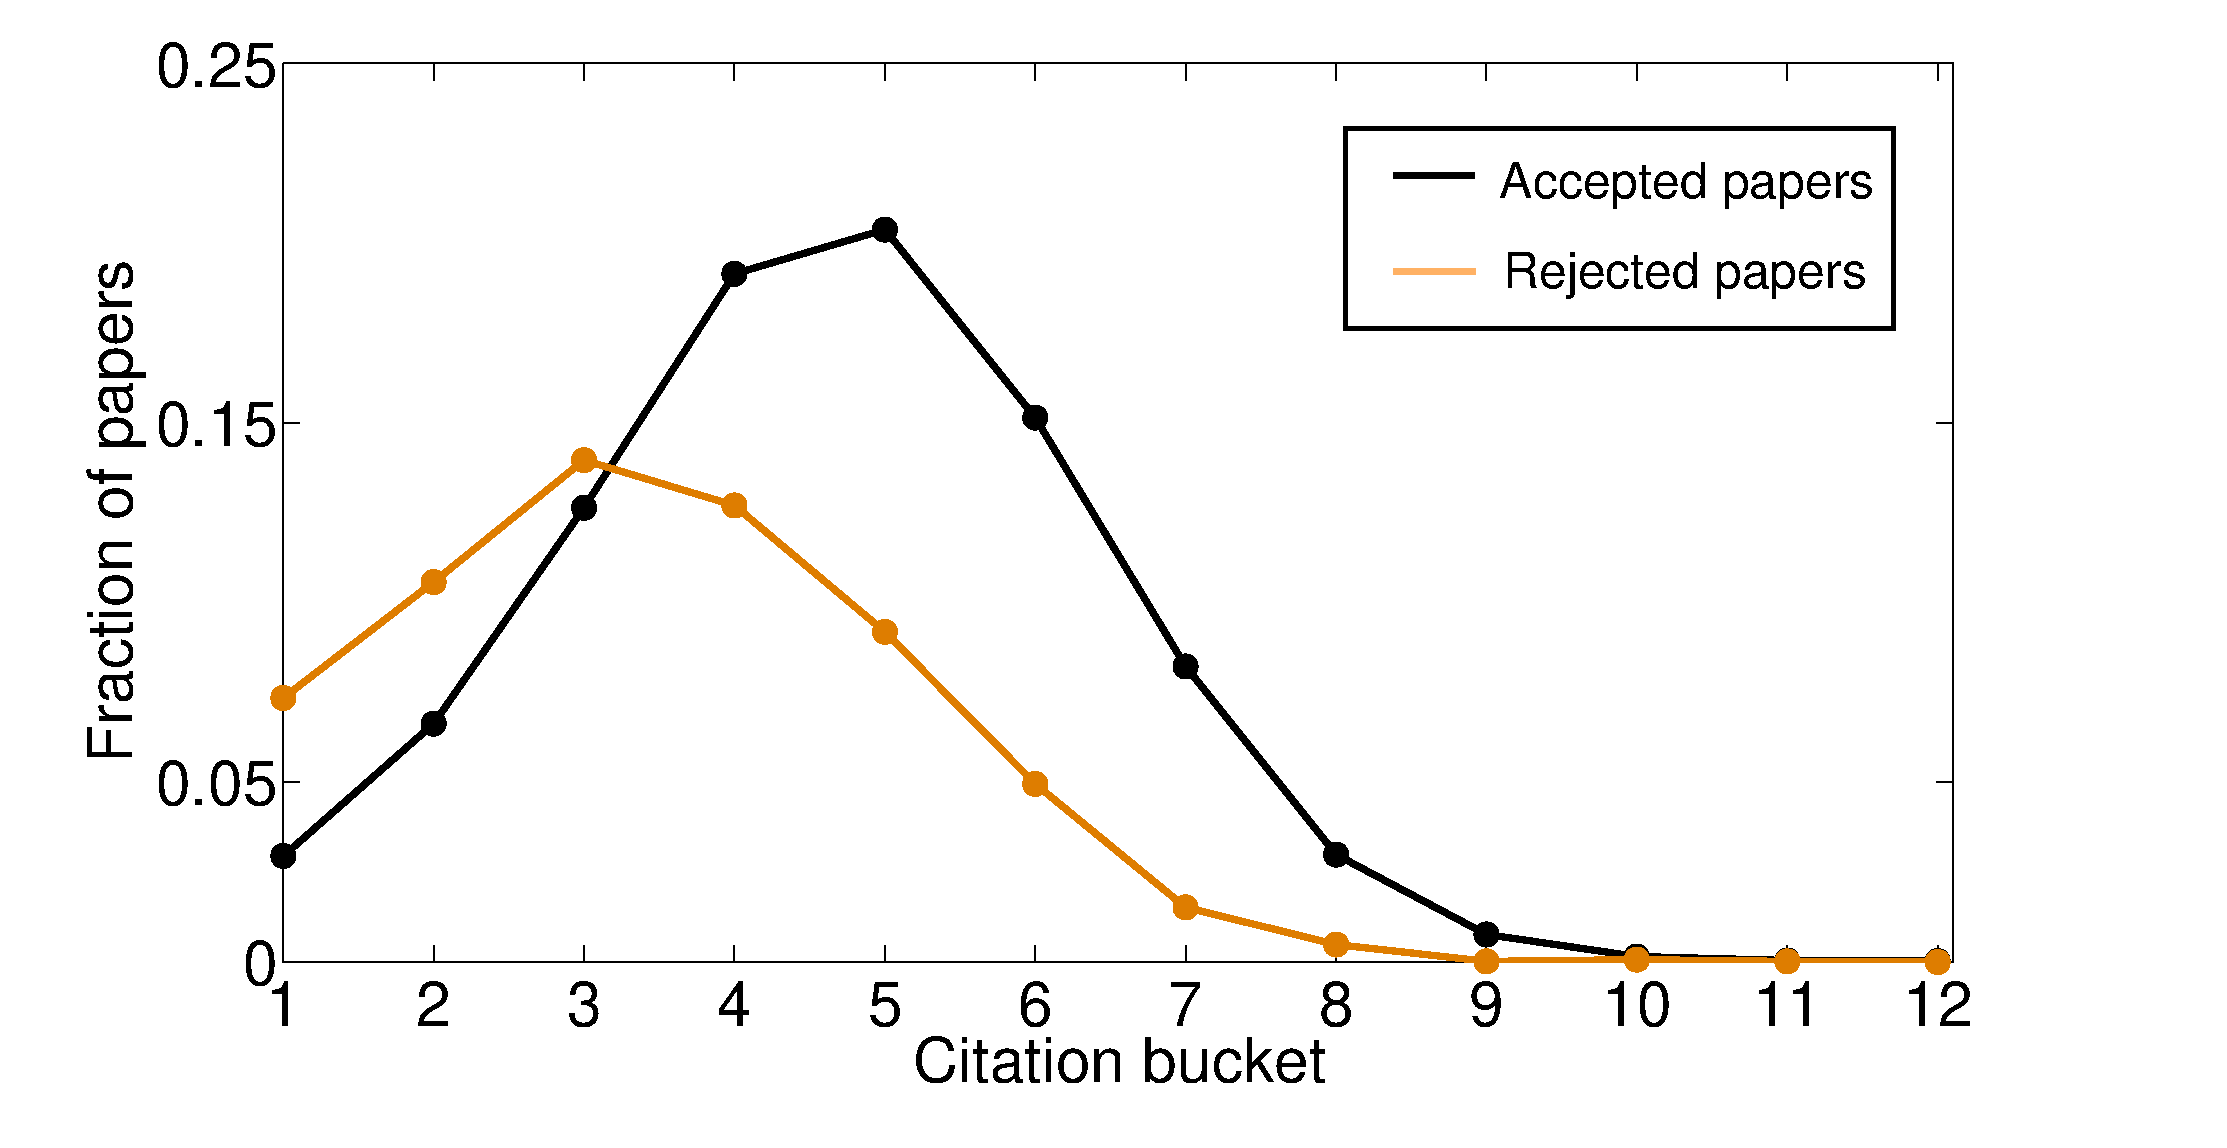
\includegraphics[scale=0.12]{./texfiles/Chapter_4/jcdl/figures/citation_bucket_frac_paper} & 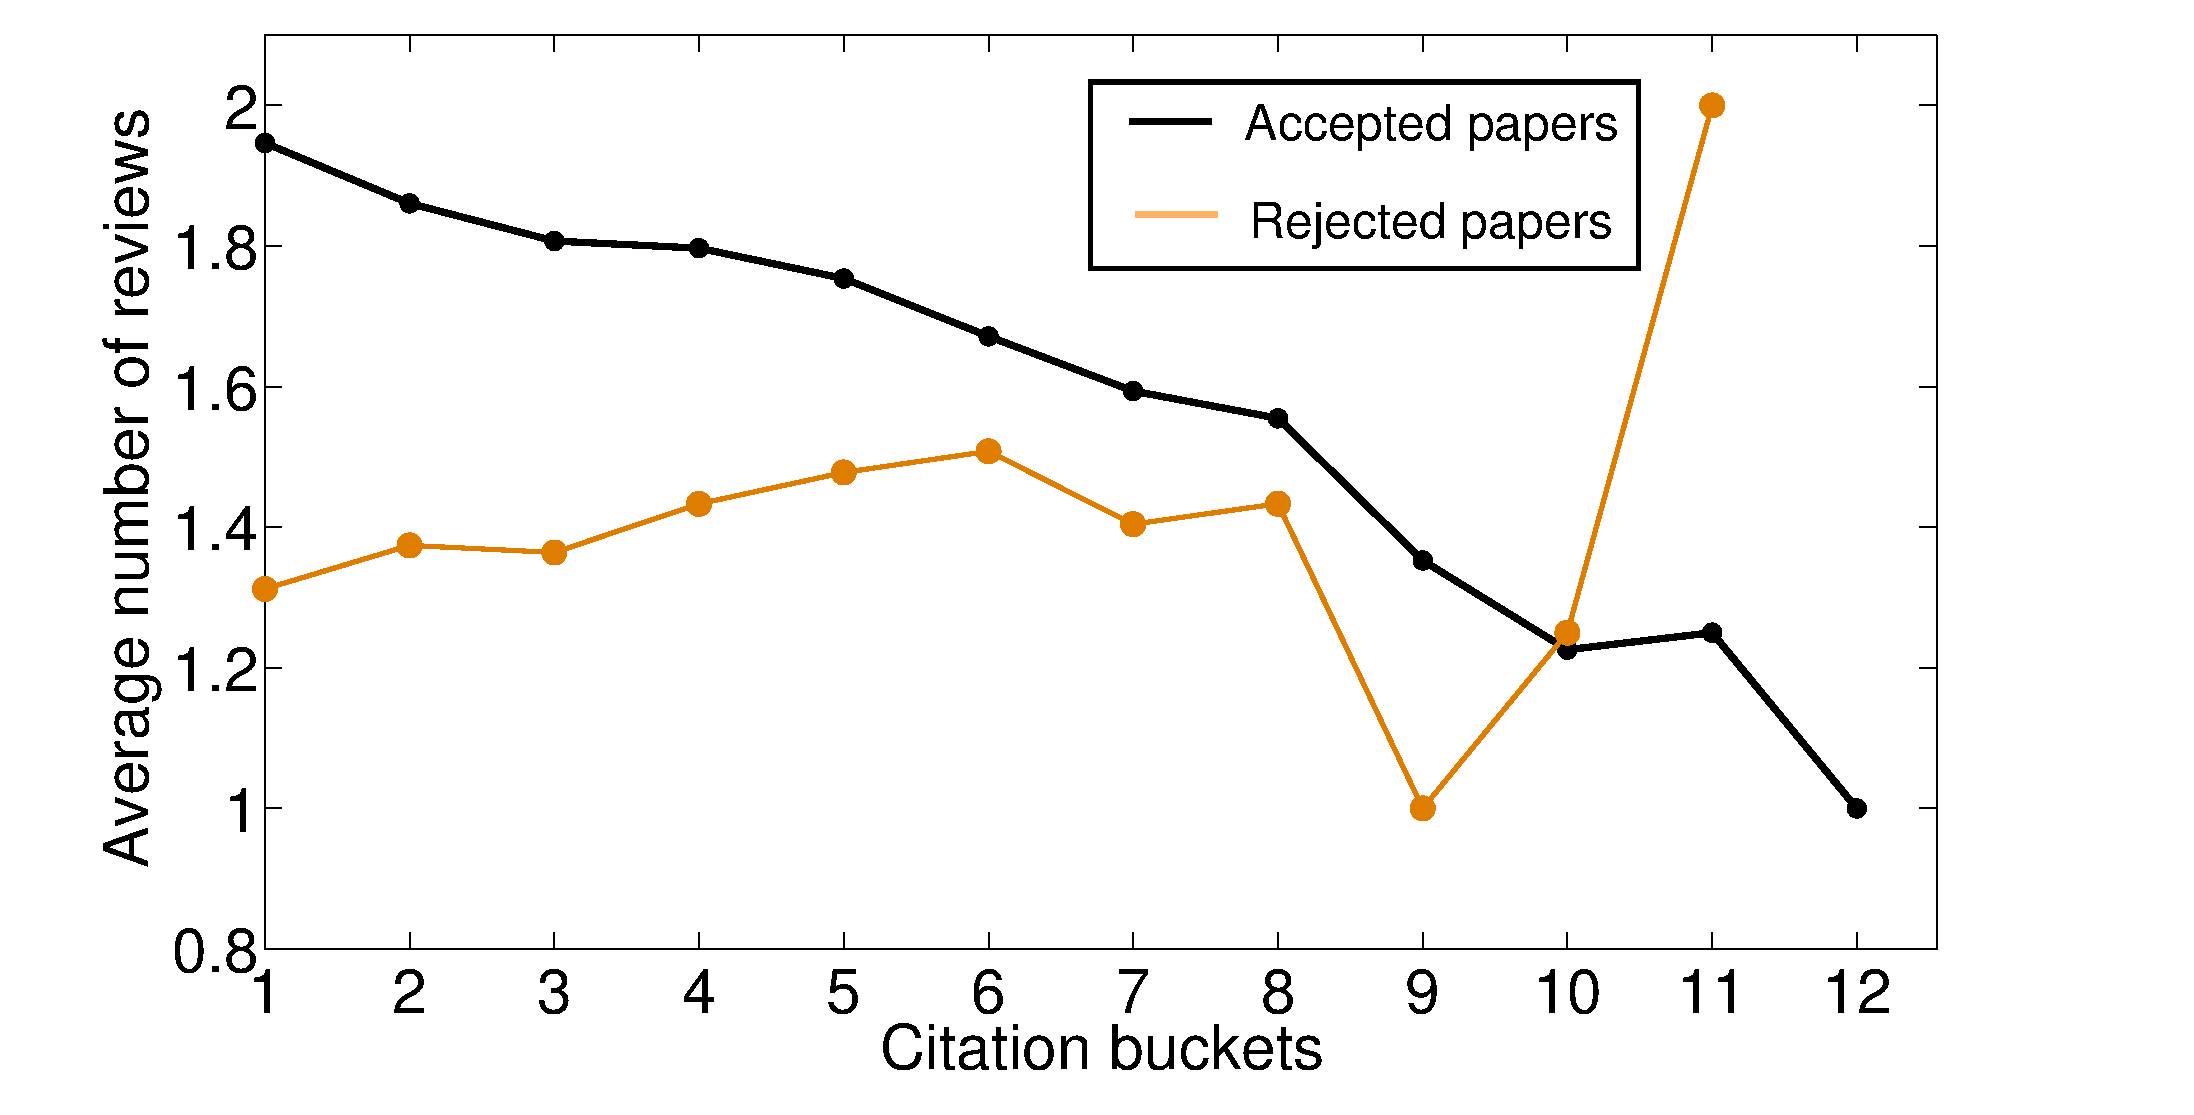
\includegraphics[scale=0.12]{./texfiles/Chapter_4/jcdl/figures/citation_bucket_reviews_all-eps-converted-to.pdf} & 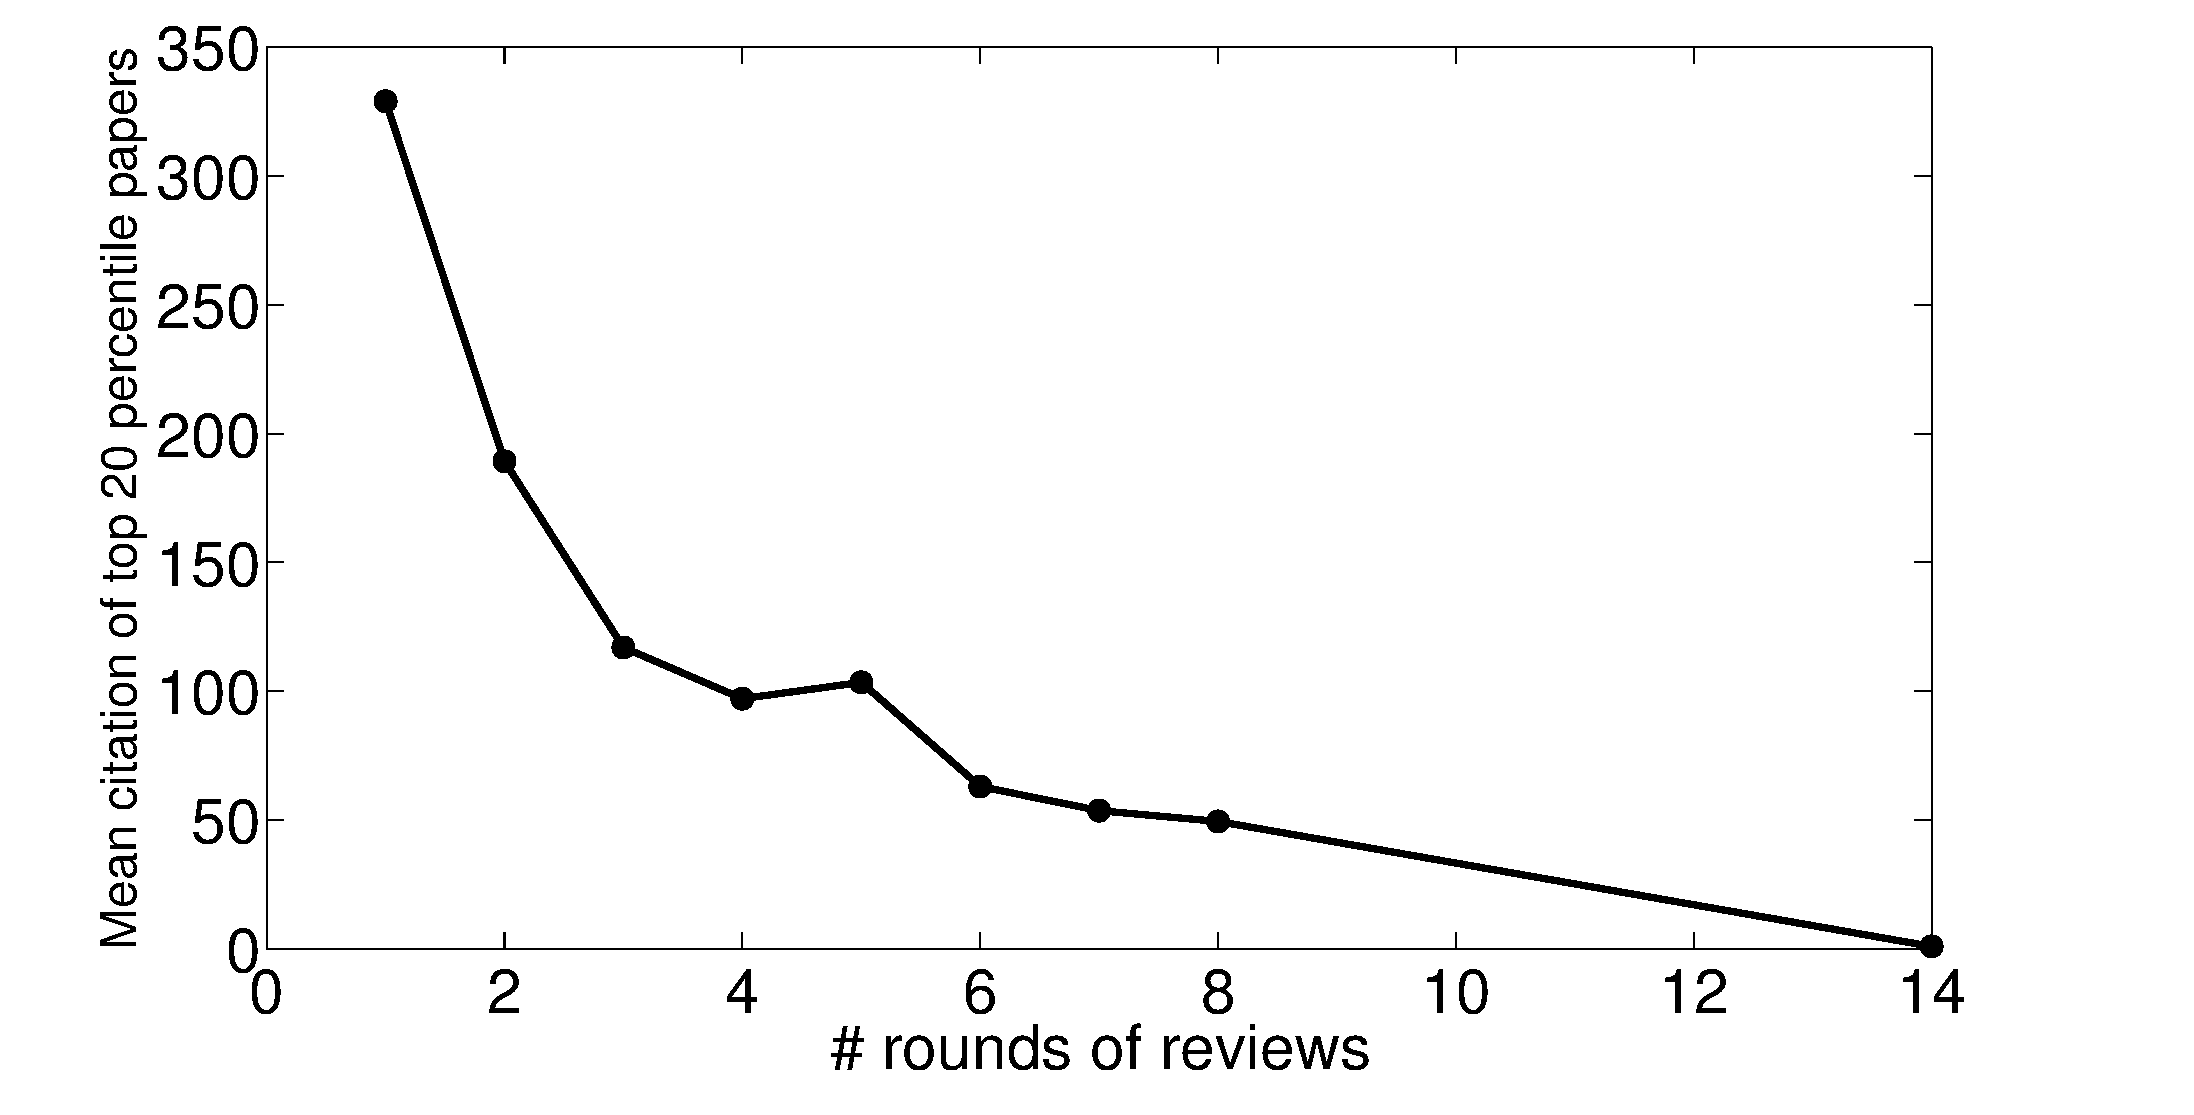
\includegraphics[scale=0.12]{./texfiles/Chapter_4/jcdl/figures/cit_rnd_rev-eps-converted-to.pdf}
 \end{tabular}
  \caption{{\bf (Left)} Fraction of accepted and rejected papers in different citation buckets. {\bf (Middle)} Average number of reviews for accepted and rejected papers in different citation buckets. For both {\bf (Left)} and {\bf(Middle) } bucket sizes are in increasing powers of 2. E.g. $\leq 1$, $2$, ($>2$ and $\leq 4$) and so on. {\bf (Right)} Average citation of the top 20 percentile  papers for a given number of rounds of review request.}
   \label{fig4}
   \vspace{4mm}
 \end{figure*}


We next check whether the {\bf review rounds} improve the quality of the paper. To this aim we segregate the papers based on the number of citations into different buckets and for each bucket we calculate the average number of reviews the papers received in that bucket. The bucket sizes are again in increasing powers of 2. Typically, the buckets are $\leq 1$, $2$, $(>2$ and $\leq 4)$ and so on. We plot the results in figure~\ref{fig4} {\bf (Middle)}. We observe that for accepted papers, the low cited ones on average tend to get accepted after more rounds of reviews while the high cited ones undergo lesser rounds of reviews before getting accepted. It can hence be concluded that going through the review process multiple times does not necessarily improve the quality of the papers much that are eventually accepted. For the rejected papers we observe a contrasting trend indicating that the review process indeed helped in improving the quality of the paper in the long run possibly enhancing the chances of its acceptance at a different venue later. For the accepted papers we further classify them based on the number of reviews they received and calculate the average citations of the top 20 percentile papers (ranked by citations) in each class (refer to figure~\ref{fig4} {\bf (Right)}). We observe that the average citation drops as the number of reviews increases further suggesting that papers accepted after higher number of reviews often fail to create a high citation impact. This indicates that the number of rounds of review could be an indicator of the long-term citation of the paper. 

\begin{figure}
\centering
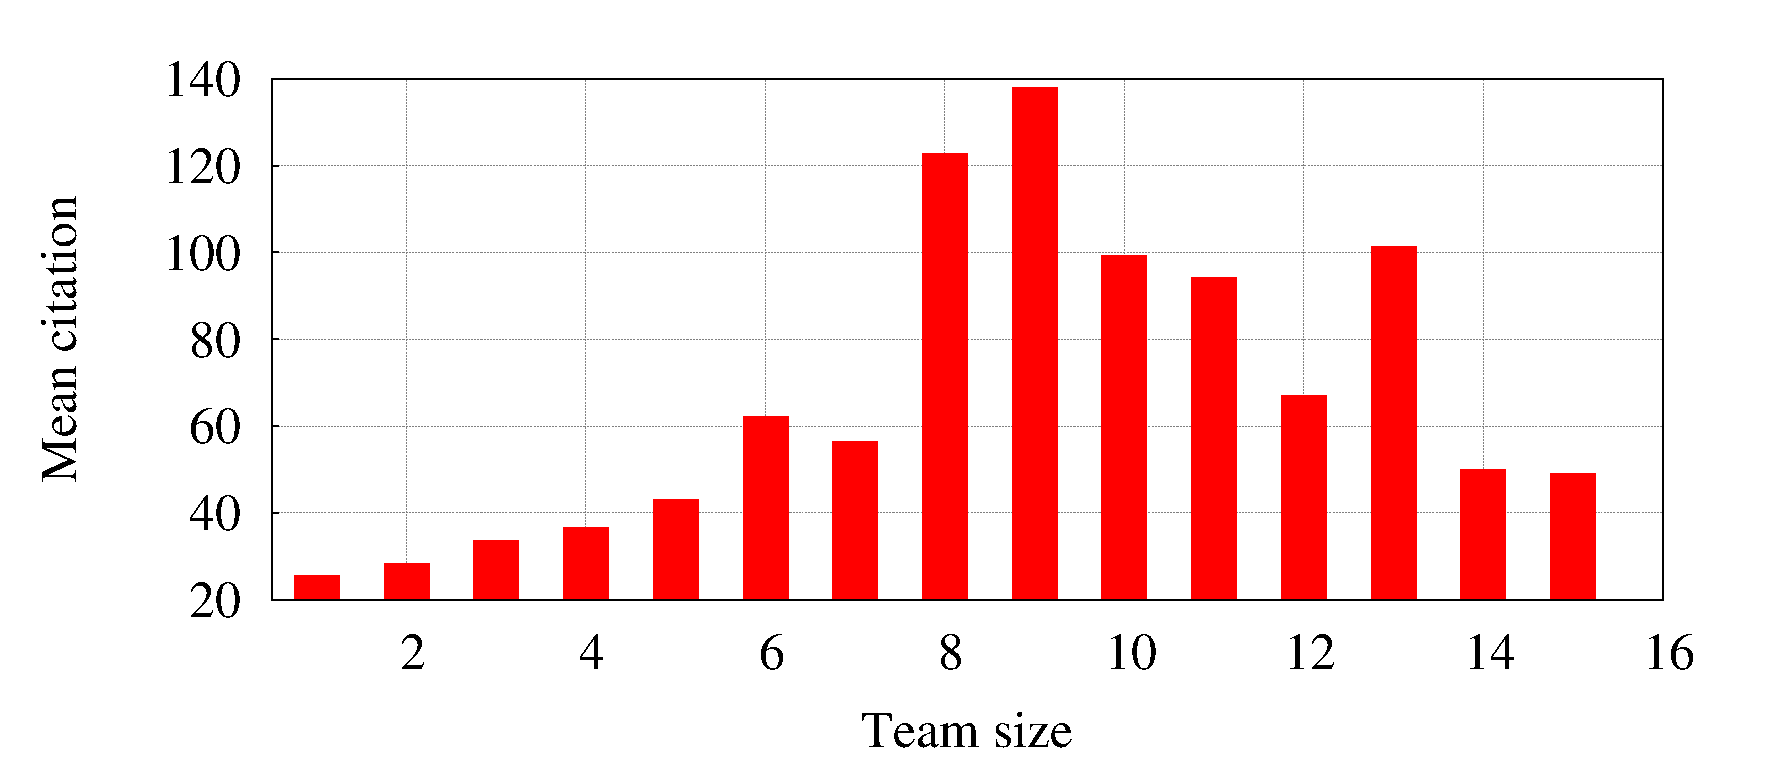
\includegraphics[scale  = 0.25]{./texfiles/Chapter_4/jcdl/figures/team_citation}
\caption{\label{team:citation} Average citation versus team size. Note that we segregate the papers based on the teams size and calculate the average citation.}
\vspace{4mm}
\end{figure}


\subsubsection*{Team size (TS)}
The authors in~\cite{chakraborty2014towards} hypothesized that there exits an optimal team size for which the citations received by the paper is maximum. We hence segregate the papers based on the team size and calculate the mean citation of the papers. We observe that team size 9 (refer to figure~\ref{team:citation}) is the optimal as the papers with 9 authors gets more citation on average.

\medskip